\documentclass[11pt]{beamer}
%\usetheme{Pittsburgh}
\usepackage[utf8]{inputenc}
\usepackage[english]{babel}
\usepackage{amsmath}
\usepackage{amsfonts}
\usepackage{amssymb}
\author{Jonas Ackermann and Lasse Schuirmann}
\title{Discrete Inverse Problems - Solving Real Problems}
%\setbeamercovered{transparent} 
%\setbeamertemplate{navigation symbols}{} 
%\logo{} 
%\institute{} 
%\date{} 
%\subject{}
\begin{document}


\begin{frame}
\titlepage
\end{frame}


\begin{frame}
\tableofcontents
\end{frame}


\begin{frame}{Barcode Reader}
\begin{center}

\includegraphics[scale=0.5]{Barcode_example.PNG} 
\end{center}
\end{frame}


\begin{frame}{Barcode Reader}
\begin{center}
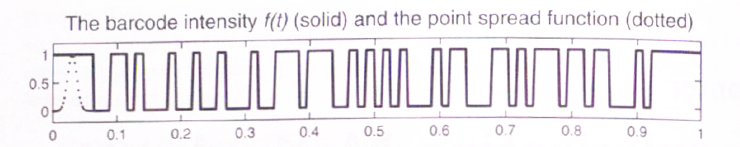
\includegraphics[scale=0.5]{Barcode_f.PNG} 
\end{center}
\end{frame}


\begin{frame}{Modellierung des Barcode Readers}
\begin{center}
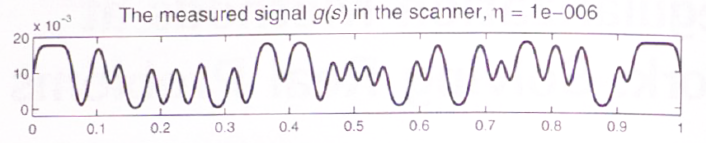
\includegraphics[scale=0.5]{Barcode_g.PNG} 
\end{center}
\end{frame}


\begin{frame}{Modellierung des Barcode Readers}
\[g(s) = \int\limits_{0}^1 f(t) \cdot h(s-t) dt = \int\limits_{0}^1 f(t) \cdot e^{-\left(s-t \over \varsigma\right)^2} dt, \, \, \, \, \, \, 0 \leq s \leq 1 \]
\end{frame}


\begin{frame}{Barcode Reader: Faltung}
Entspricht einer Faltung $\rightarrow$ Invers: Dekonvolution (Entfaltung) 
\end{frame}


\begin{frame}{Barcode Reader: Diskretisierung}

\end{frame}

\begin{frame}{Barcode Reader: Rekonstruktion}
\begin{center}
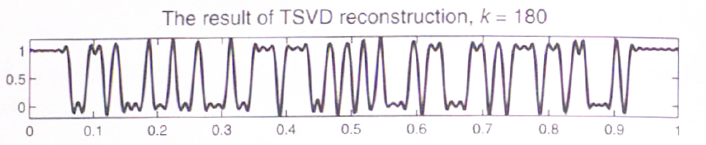
\includegraphics[scale=0.5]{Barcode_TSVD.PNG} 
\end{center}
\end{frame}

\end{document}
